\chapter{Introducción}

La adopción de arquitecturas basadas en contenedores y orquestadores como Kubernetes ha transformado la forma en que se desarrollan y despliegan aplicaciones en entornos cloud y corporativos. Este paradigma permite automatizar la gestión del ciclo de vida de las aplicaciones, mejorar la escalabilidad y facilitar la integración de prácticas de desarrollo modernas. Sin embargo, esta evolución tecnológica también introduce nuevos desafíos en materia de seguridad, especialmente en entornos donde los despliegues se realizan de forma automatizada y continua.

En este contexto surge el enfoque DevSecOps, cuyo objetivo es integrar la seguridad dentro del propio ciclo de vida del desarrollo de software, en lugar de tratarla como una fase posterior al despliegue. Este modelo promueve la automatización de controles de seguridad dentro de los pipelines de integración y despliegue continuo, permitiendo detectar vulnerabilidades, aplicar políticas de seguridad y garantizar configuraciones seguras desde las primeras fases del desarrollo.

El presente Trabajo de Fin de Máster se centra en la implementación de un entorno DevSecOps completo sobre Kubernetes, integrando herramientas de Integración Continua (GitHub Actions) con análisis automatizado de vulnerabilidades mediante herramientas como Trivy y Sysdig Secure. Asimismo, se implementará un modelo de Despliegue Continuo basado en GitOps utilizando ArgoCD, permitiendo gestionar la infraestructura y los despliegues de forma declarativa a través de repositorios Git.

Adicionalmente, se incorporará el uso de Kyverno como motor de políticas de seguridad basado en Policy-as-Code, permitiendo aplicar controles automáticos sobre los manifiestos de Kubernetes durante el proceso de despliegue.

El núcleo del proyecto se basa en el uso de Admission Controllers, concretamente Kyverno, para aplicar políticas de seguridad de forma declarativa dentro del clúster de Kubernetes. A diferencia de los enfoques tradicionales que únicamente bloquean configuraciones inseguras, este trabajo explorará el uso de políticas de tipo mutating, capaces de corregir automáticamente configuraciones inseguras en los manifiestos YAML en tiempo de despliegue.

Finalmente, el proyecto incluirá un análisis comparativo entre Kyverno y OPA Gatekeeper, evaluando sus capacidades en la implementación de políticas de seguridad en Kubernetes, su facilidad de uso, curva de aprendizaje y eficacia en entornos de producción.

La Figura \ref{fig:arquitectura-devsecops} muestra una visión general de la arquitectura DevSecOps implementada en este trabajo, donde se integran los procesos de desarrollo, análisis de seguridad, despliegue continuo y aplicación de políticas dentro de un entorno Kubernetes.

\begin{figure}[H]
\centering
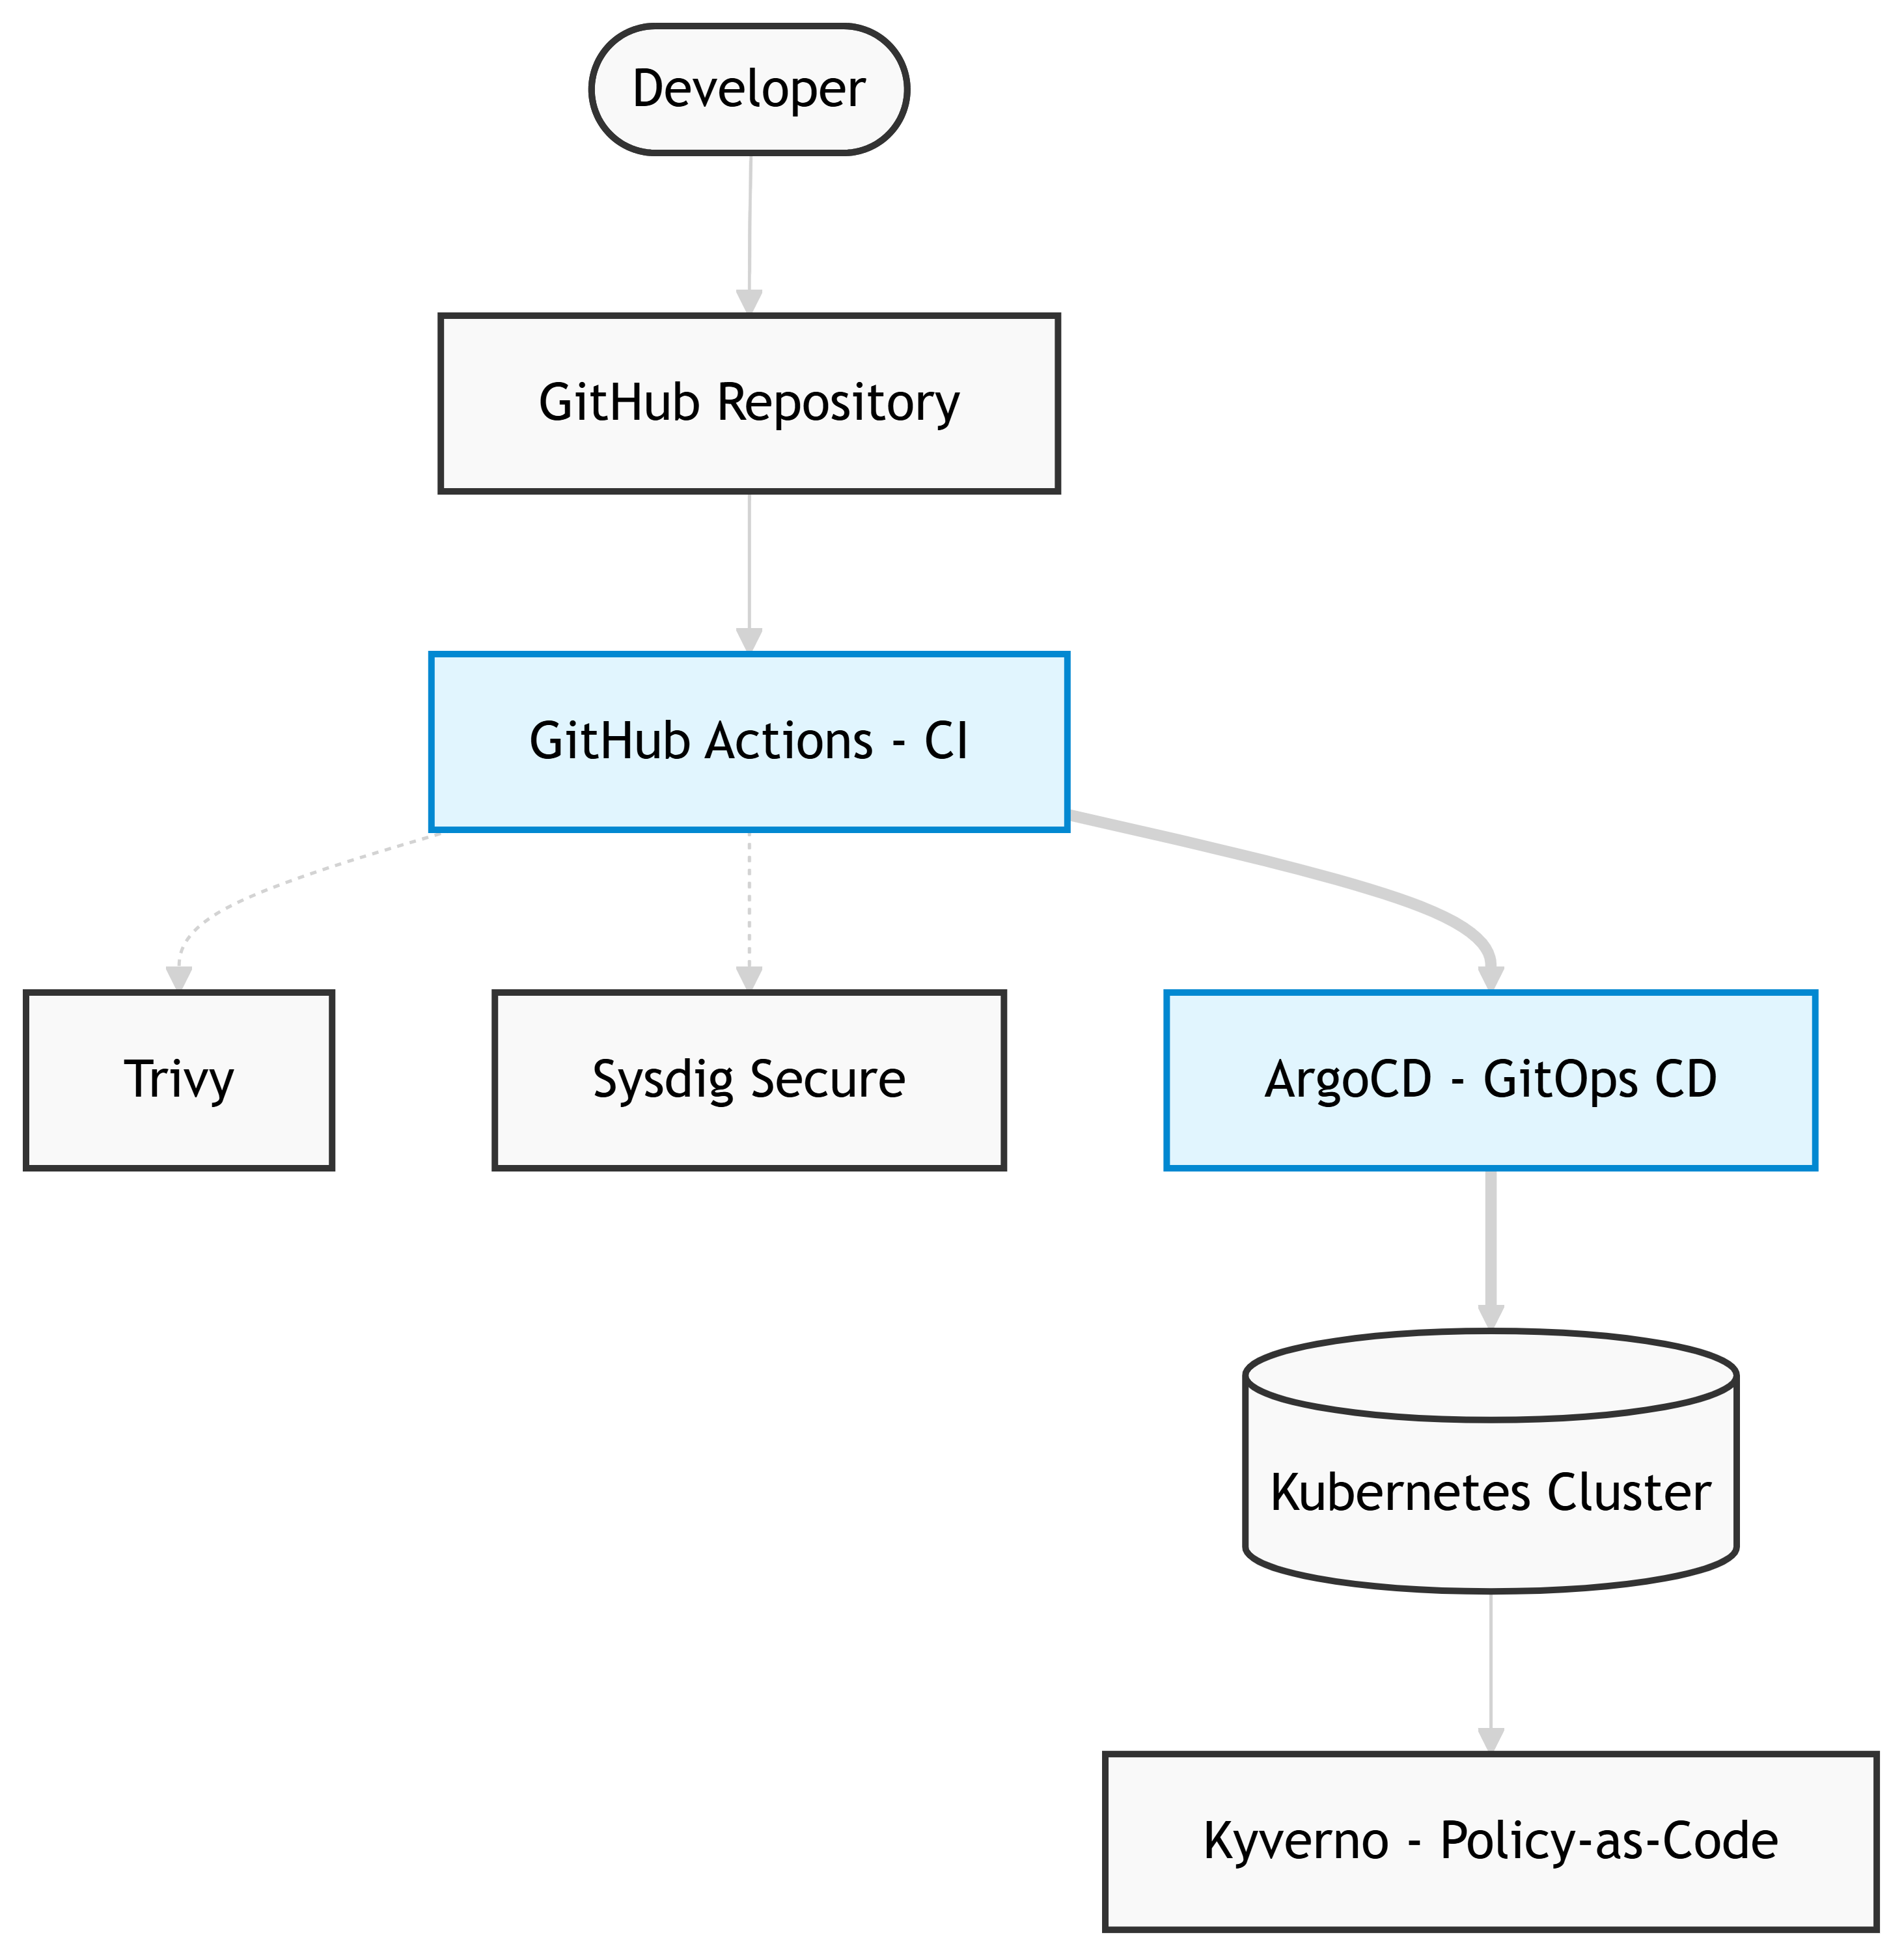
\includegraphics[width=0.5\linewidth]{images/arquitectura_DevSecOps.png}
\caption{Arquitectura general del entorno DevSecOps}
\label{fig:arquitectura-devsecops}
\end{figure}
